\documentclass[a4paper,11pt]{jsarticle}


% 数式
\usepackage{amsmath,amsfonts}
\usepackage{bm}
\usepackage{physics}
% 画像
\usepackage[dvipdfmx]{graphicx}
% ローマ数字
\usepackage{otf}
% 単位
\usepackage{siunitx}
% 表
\usepackage{multirow}
% 化学反応
\usepackage[version=4]{mhchem}

\begin{document}

\title{理論演習 研究内容}
\author{齋藤駿一}
\date{\today 作成}
\maketitle

手探りでいくつかのモデルを作って試した.

\section{細胞成長モデル(濃度ベース)}
\subsection{概要}
6月9日に発表した粒子数ベースのモデルでは,何度か「分裂」を繰り返して至る最終的な状態(終状態)が見づらかった.
また,反応速度が体積に細かく依存するため,終状態は振動していた.

\begin{figure}[htbp]
  \centering
  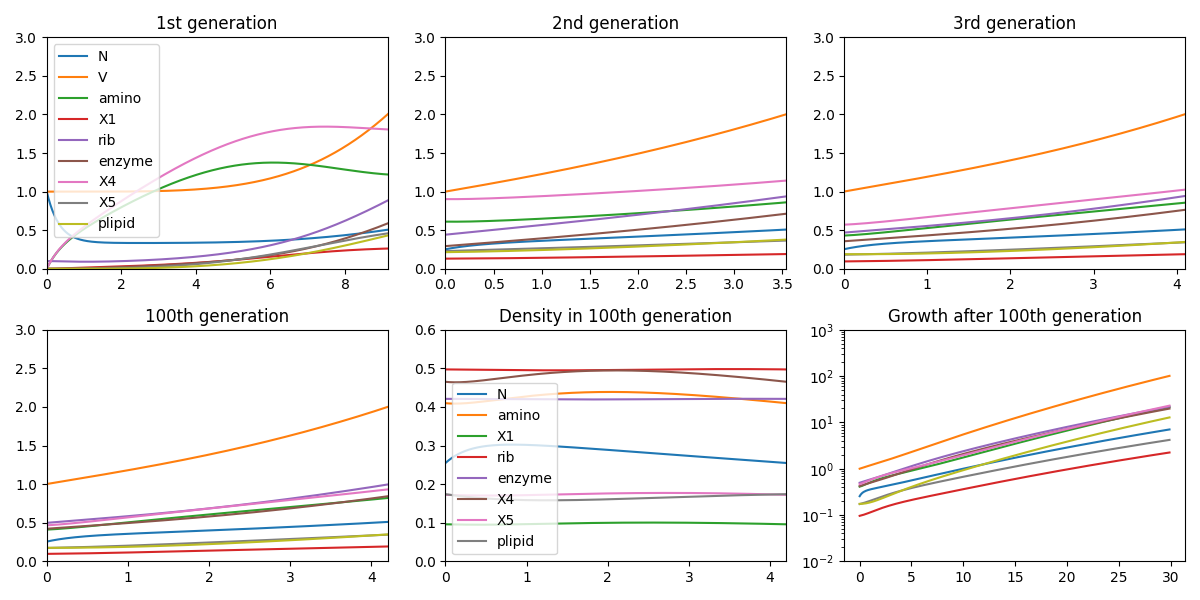
\includegraphics[width=\columnwidth]{cell_100gen.png}
  \caption{細胞成長モデル(粒子数ベース)の計算結果.先週発表した.}
  \label{fig:cell1}
\end{figure}

そこで,モデルを濃度ベースにして書き直し,反応速度から体積依存性を除いた.加えて,栄養濃度は一定として変数から外した.
その結果,終状態では全成分が定常濃度となった.


また,「分裂」の際に二項分布に従って粒子数がゆらぐ状況\footnote{各粒子が2個の娘細胞に半々の確率で分配される状況を想定している.}を考え,シミュレーションした.
その結果,リボソームが枯渇しない限り成長にあまり影響はないことが分かった.

\subsection{設定}
今回も引き続き図\ref{fig:cell2_set}の化学反応系を考えた.
ただし,栄養濃度は一定($n=\mathrm{const.}$)とした.

\begin{figure}[htbp]
  \centering
  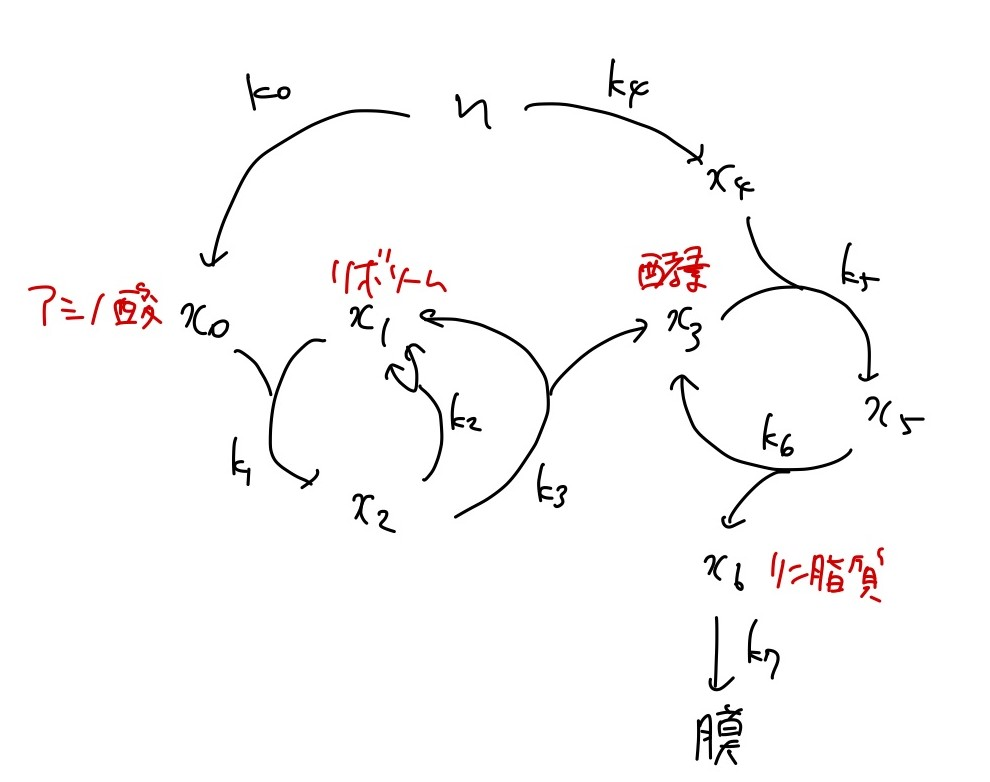
\includegraphics[width=8cm]{cell2_set.jpg}
  \caption{細胞成長モデル(濃度ベース)で仮定した化学反応系の概略図.}
  \label{fig:cell2_set}
\end{figure}

各化学反応による成分の濃度変化は,反応速度定数$k_i\,(i=0,\cdots,7)$と反応物の濃度の積で書いた(質量作用の法則).
また,体積の増大量はリン脂質$x_6$の消費量に比例すると考えて
\begin{equation}
  \frac{dV}{dt} = g k_7 x_6
\end{equation}
とし,$V$は1から2までしか変化しないので,成長速度を
\begin{equation}
  \mu = \frac{g k_7 x_6}{V} \approx gk_7 x_6
\end{equation}
とした.
各成分の濃度は,この成長速度によって希釈されるとした.


\subsection{計算内容と結果}

まず,反応速度は$k_2=0.5$\footnote{後述するゆらぎを入れた計算で「リボソームが無くなって成長が止まる」状況を作りやすくするため,リボソーム生成を遅くしている.},そのほかを$k_i=1(i\neq 2)$とし,栄養濃度は$n=1$とした.

次に,初期値を適当に$V=1, x_1=1, x_i=0(i\neq 1)$ととり,$V>2$となるまで時間発展させた.
はじめて$V>2$になった時点で,成分濃度を保って体積を半分にする操作(「分裂」と呼ぶことにする)を挟み,引き続き時間発展させた.
その後も$V$が2を超えるたびにこの操作を繰り返した.
その結果,10周期ほどで定常濃度に収束した.

次に,この定常濃度を改めて初期値に取り直した.
そしてこれ以降,「分裂」の際に粒子数が二項分布(numpy.random.binomialを用いた)に従ってゆらぐように設定した.
ここで言う粒子数とは,細胞の体積を特徴付けるパラメータ$V_0$を各成分の濃度に乗じ,小数部分を切り捨てて得られる整数値である.
これを40周期繰り返し,分裂直後の体積と各成分濃度の変動を確認した.
その結果,$V_0=30$程度かそれ以上のサイズでは最後の周期までもつが,$V_0=15$程度かそれ未満のサイズでは途中で成長が止まることがあった.
成長停止の原因は,大きなゆらぎによってリボソームが枯渇し,自己触媒ができなくなって全成分が希釈されるためである.

\begin{figure}[htbp]
  \centering
  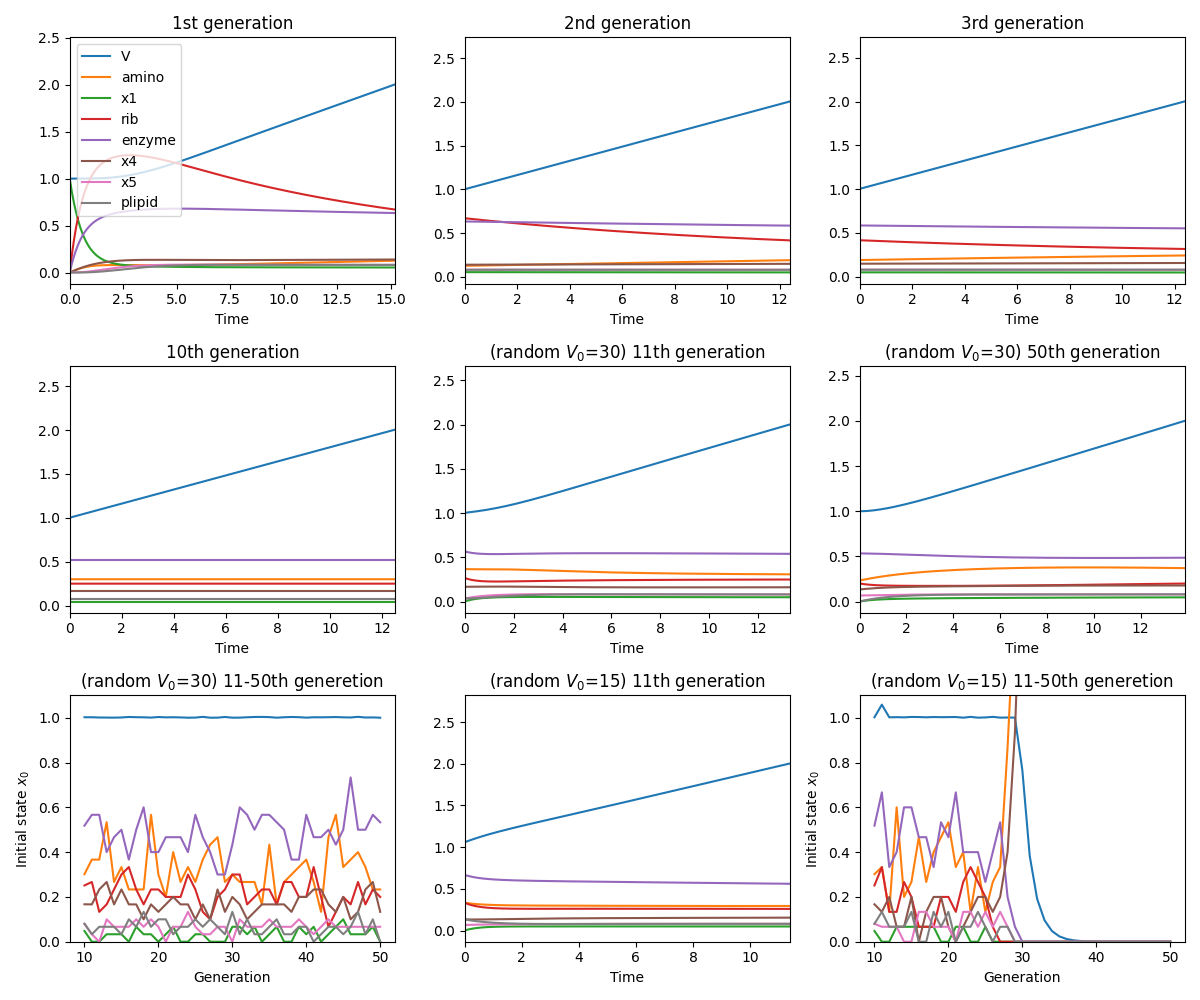
\includegraphics[width=\columnwidth]{cell2.png}
  \caption{細胞成長モデル(濃度ベース)の計算結果.最初の10周期で「分裂」を繰り返したところ,定常状態へ収束した.11周期目からは「分裂」に伴って粒子数が二項分布に従ってゆらぐとして計算した.このとき,濃度から粒子数への変換に用いた細胞体積として$V_0 = 30,15$の2通りを考えた.$V_0=15$ととった場合,途中でリボソームが枯渇して成長が止まったが(図右下),リボソームが枯渇した後の計算結果には意味がないので無視して良い.(計算が続いているのは「分裂」のプログラムの仕様である.)}
  \label{fig:cell2}
\end{figure}


\section{二個のautocatalytic cycleが別々に回るモデル}
\subsection{概要}
上で見たautocatalytic cycleは全成分が定常濃度に収束した.
これはかなり典型的な性質のようだったので,その例外にあたるcycleを考えた.
具体的には,2つの独立なautocatalytic cycleを異なる反応速度で回し,遅いcycleだけが膜形成に寄与すると仮定した.
このとき,もう片方の速いcycleに含まれる成分の濃度はどこまでも増加した.
ただし,速いcycleの成分が遅いcycleの成分に変わる化学反応が存在すれば,遅いcycleが速く回るようになり,全成分定常濃度が実現した.

\subsection{設定}
独立に回る簡単なautocatalytic cycleを2つ用意する.
\begin{align}
  \ce{N + X_1 ->[$k_1$] X_2 ->[$k_2$] 2X_1}\\
  \ce{N + X_3 ->[$k_3$] X_4 ->[$k_4$] 2X_3}
\end{align}
このうち下のcycleの方が速いと仮定する.
ここでは$k_1=k_2=10, k_3=k_4=11$とした.
加えて,$i=1,2,  j=3,4$に対して,次の反応も考える.
\begin{align}
  \ce{X_i ->[$k_{ij}$] X_j}  \\
  \ce{X_j ->[$k_{ji}$] X_i} 
\end{align}
ここでは$k_{31}$以外ゼロとする.
また,$X_1$が反応速度$k_g$で消費されて膜が形成されると考え,
\begin{equation}
  \frac{dV}{dt} = g k_g X_1
\end{equation}
とした.
希釈と「分裂」については先ほどと同様である.
ここでは栄養濃度を$n=1$,$X_1$の消費速度を$k_g = 1$,成長速度を$g=1$とした.

\subsection{結果}
$k_{31}=0$のとき,$X_3$と$X_4$の濃度は発散した(図\ref{fig:cp0}).
$k_{31}=1$のとき,$X_3$と$X_4$の濃度は収束した(図\ref{fig:cp1}).
また,$k_{31}$の代わりに$k_{32}, k_{41}, k_{42}$でも同じく収束した(図\ref{fig:cp2}).
このことから,速いcycleから遅いcycleへ向かうような反応があると全成分定常濃度が実現することが分かった.

\begin{figure}[htbp]
  \centering
  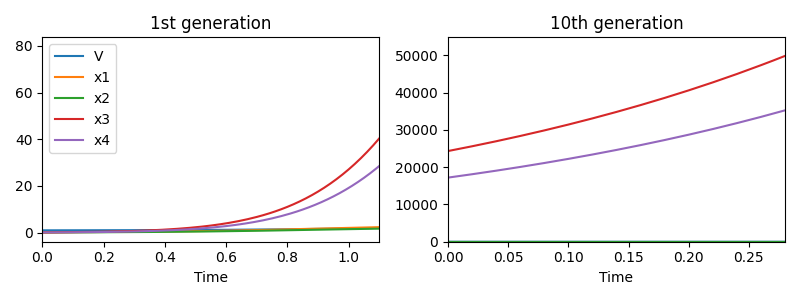
\includegraphics[width=10cm]{couple_pure_k31=0.png}
  \caption{$k_{31}=0$の場合の計算結果.収束しなかった.}
  \label{fig:cp0}
\end{figure}

\begin{figure}[htbp]
  \centering
  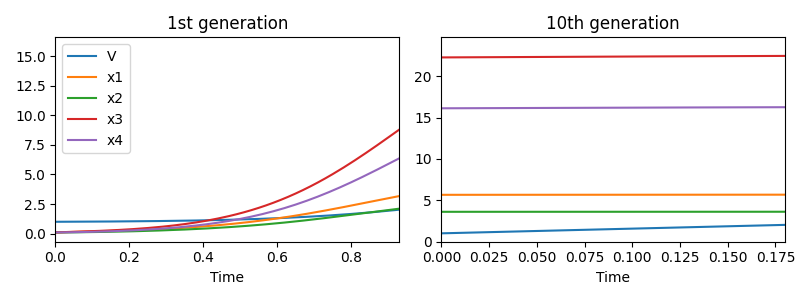
\includegraphics[width=10cm]{couple_pure_k31=1.png}
  \caption{$k_{31}=1$の場合の計算結果.収束した.}
  \label{fig:cp1}
\end{figure}

\begin{figure}[htbp]
  \centering
  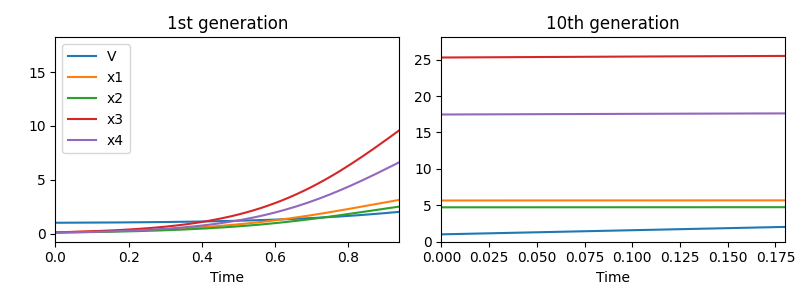
\includegraphics[width=10cm]{couple_pure_k42=1.png}
  \caption{$k_{42}=1$の場合の計算結果.$k_{31}=1$のときと定常濃度は若干異なるが,やはり収束した.}
  \label{fig:cp2}
\end{figure}

\section{Expression burstを入れたモデル}
\subsection{概要}
先週,expression burstという現象をはじめて知ったので,その効果を加味したシミュレーションを行った.
反応のモデルとしては,自己触媒する酵素が膜前駆体を形成する,というものを考えた.
ここではこの酵素の濃度がexpression burstによってゆらぐときの成長の様子を計算した.
また,burstによって細胞周期(「分裂」から次の「分裂」までの時間間隔)がゆらぐことも確認した.

\subsection{設定}
反応系は次のようなものを考えた(金子邦彦『普遍生物学』p.59にあった姫岡先生のモデルを参考にした.).
$x_1$は酵素E,$x_4$は膜前駆体Mを想定している.
今回は逆反応も考えた.

\begin{align}
  &\ce{N1 + E <=> N1E <=> 2E}\\
  &\ce{N2 + E <=> N2E <=> M + E }
\end{align}

体積変化は膜前駆体の消費速度$k_0$を用いて
\begin{equation}
  \frac{dV}{dt} = g k_0 x_4
\end{equation}
で与え,これによる希釈も考える.

加えて,酵素Eの増加する要因として,自己触媒のほかに,対応するmRNAからの翻訳による分も考えた.
翻訳による増加は,expression burstを想定する.
具体的には,計算の各ステップ(刻み幅$dt$)において確率$p$で翻訳が起こり,酵素Eの濃度は臨時的に$(b/p)dt$だけ不連続に増えるとした.
また,この臨時流入の期待値を0にするために,酵素Eは微小時間$dt$の間に$bdt$だけ定常的に分解するとした.
ただし,酵素濃度の計算結果が負になってしまったときは,ゼロで置き換えるようにした.

栄養濃度と成長速度はそれぞれ$n_1=n_2=1, g=1$とした.
また,$dt=0.01, p=0.05, b=5$として臨時流入が$1$になるようにし,順方向の反応速度定数はすべて$1$,逆方向の反応速度定数は$\ce{N1E <- 2E}$だけ$0.1$,その他は$0.5$とした.

\subsection{結果}
計算の結果,図\ref{fig:burst}が得られた.
また,定常濃度での細胞周期は$2.53$だったが,expression burstが入ってからの細胞周期は$1.83-2.24$だった.
しかし,乱数の種を変えると細胞周期が$3.91$にまで伸びることもあったので,「expression burstによって細胞周期が短くなる」というわけではなさそうだった.

\begin{figure}[htbp]
  \centering
  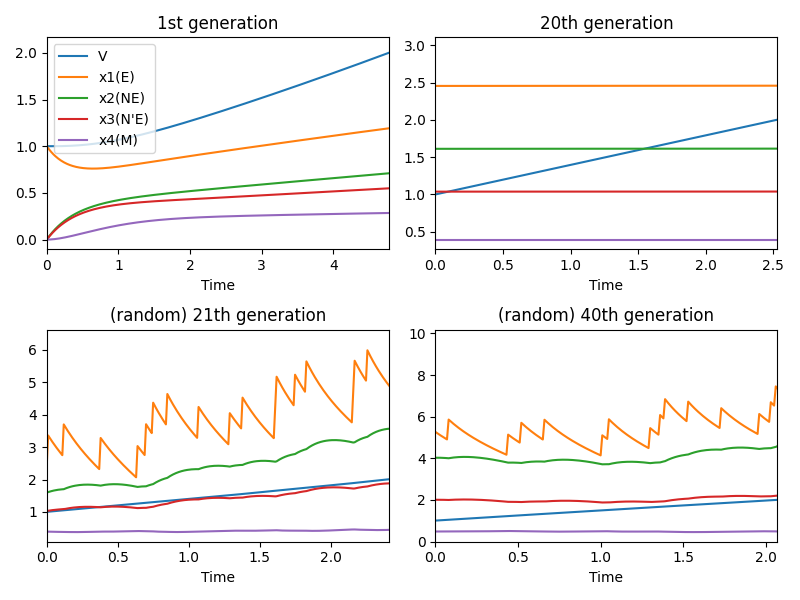
\includegraphics[width=10cm]{burst.png}
  \caption{Expression burstを入れたモデルの計算結果.}
  \label{fig:burst}
\end{figure}

\end{document}